\chapter{Introduzione}
\section{Gli ingredienti del machine learning}
L'obiettivo è risolvere un problema partendo da esempi di problemi già risolti.
Per parlare di \textbf{machine learning} dobbiamo avere chiari 3 concetti fondamentali:
\begin{itemize}
    \item tasks, sono una specifica di cosa vogliamo fare (classification, regression, probability estimation;
clustering,...),
    \item model, riguardano la modalità di risoluzione del task (linear, decision trees, naive Bayes, Knn,...);
    \item features, sono il modo in cui sono descritti gli esempi da utilizzare per risolvere il problema(numerical, categorical, feature construction,
feature selection,...).
\end{itemize}

\paragraph{Esempio: l'email} 
L'obiettivo è classificare un'email come spam o come ham. Al posto di analizzare il testo, utilizziamo delle features costruite su di esso. 
Qunidi in partenza abbiamo le features, che sono raggruppate in vettori, e una etichetta che può essere spam o ham. Dobbiamo scrivere una funzione che prenda in input il vettore e restituisca l'etichetta corretta.
\textbf{SpamAssassin} è un programma per individuare email spam.
Sulla sinistra ci sono degli score che sono associati alle features; se una featutures è vera, aumenta la probabilità che l'email sia spam.

\begin{figure}
    \centering
    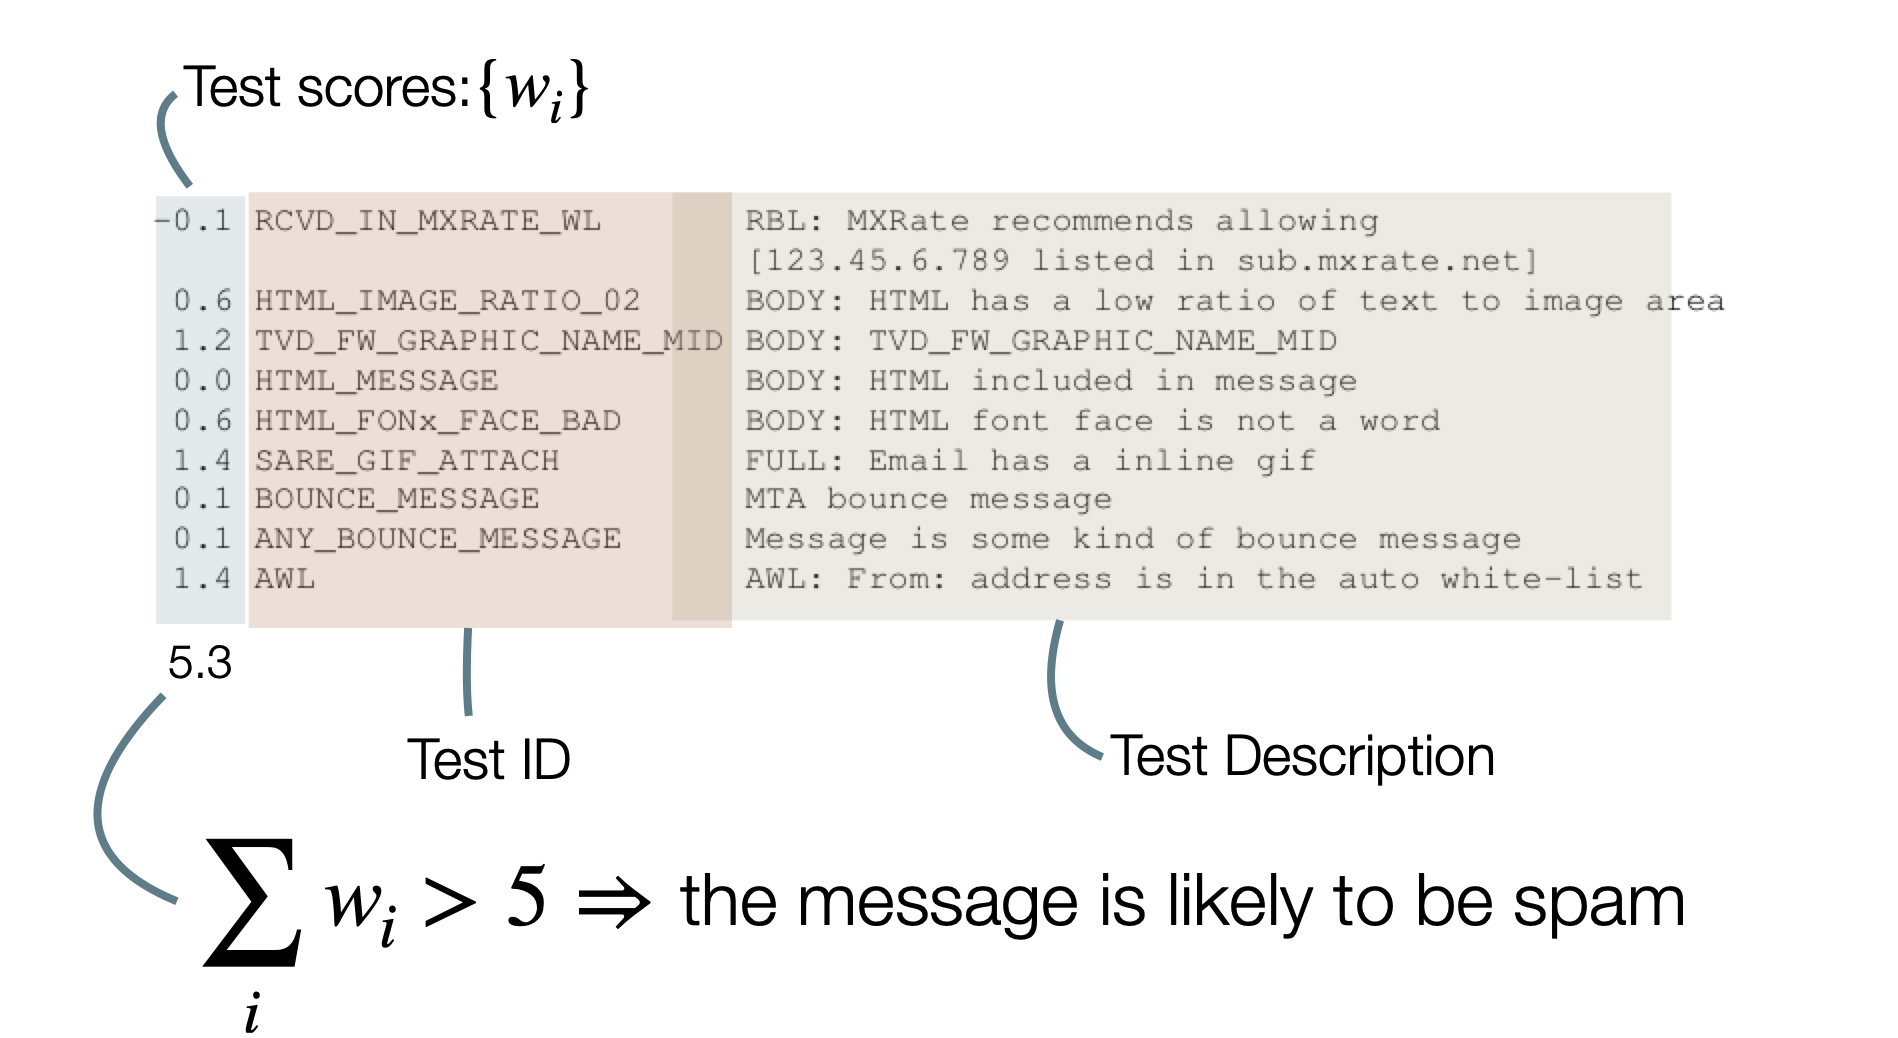
\includegraphics[scale=0.3]{images/spamAssassin.png}
    \caption{\textbf{Nota:} email \textbf{ham} è il contrario di email \textbf{spam}.}
    \label{fig:enter-label}
\end{figure}

\newpage

\paragraph{Machine Learning} \textbf{L'apprendimento automatico} è lo studio sistematico di algoritmi e sistemi che migliorano la loro \textbf{conoscenza} o \textbf{performance}(=funzione che misura quanto il modello sta facendo bene) attraverso l'\textbf{esperienza}(=esempi, features)

\begin{figure}
    \centering
    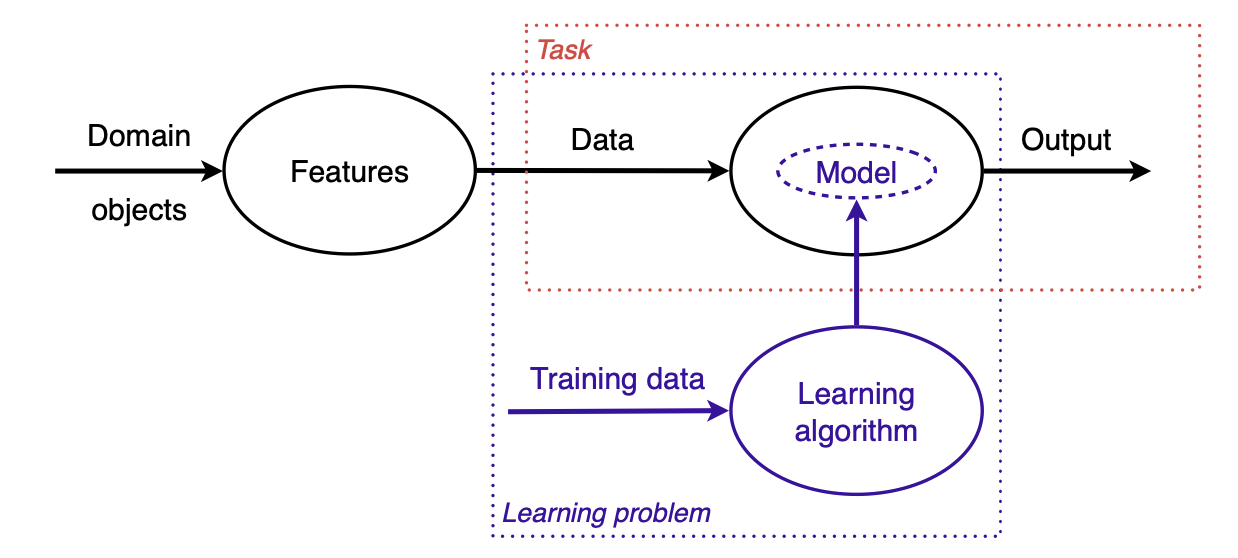
\includegraphics[scale=0.5]{images/mlModel.png}
    \caption{come il machine learning aiuta a risolvere un task}
    \label{fig:enter-label}
\end{figure}


Per risolvere un \textbf{task} devo \textbf{sfruttare un modello}, per risolvere un \textbf{problema di apprendimento} devo usare un qualche \textbf{algoritmo di apprendimento} che sviluppi un \textbf{modello} per risolverlo.

\section{Task} Ci sono sostanzialmente 2 tipi di task che si affrontano con l'apprendimento automatico: \textbf{task predittivi}  e \textbf{task descrittivi}. Nei predittivi si vuole predirre una qualche variabile a fronte delle descrizione degli esempi. I predittivi si disinguono a loro volta a seconda delle etichette che vogliamo predire:
\begin{itemize}
    \item \textbf{classificazione binaria (2 etichette) o multiclasse (più etichette)}, etichetta di tipo categorico (es. spam, ham);
    \item \textbf{regressione}, etichetta numerica;
    \item \textbf{clustering}, target nascosto.
\end{itemize}

I \textbf{task descrittivi} non hanno l'etichetta fornita, l'idea è prendere i dati forniti e fornire una descrizione di essi che sia utile a chi fa l'analisi.

\paragraph{Overfitting.} L'idea nel caso estremo è che si memorizzano troppo gli esempi e, quando si deve predirre, si tira fuori l'etichetta (se si è vista), altrimenti si va a caso. Il punto è che il modello si specializza sugli esempi forniti e non riesce a generalizzare.

\newpage
\begin{figure}
    \centering
    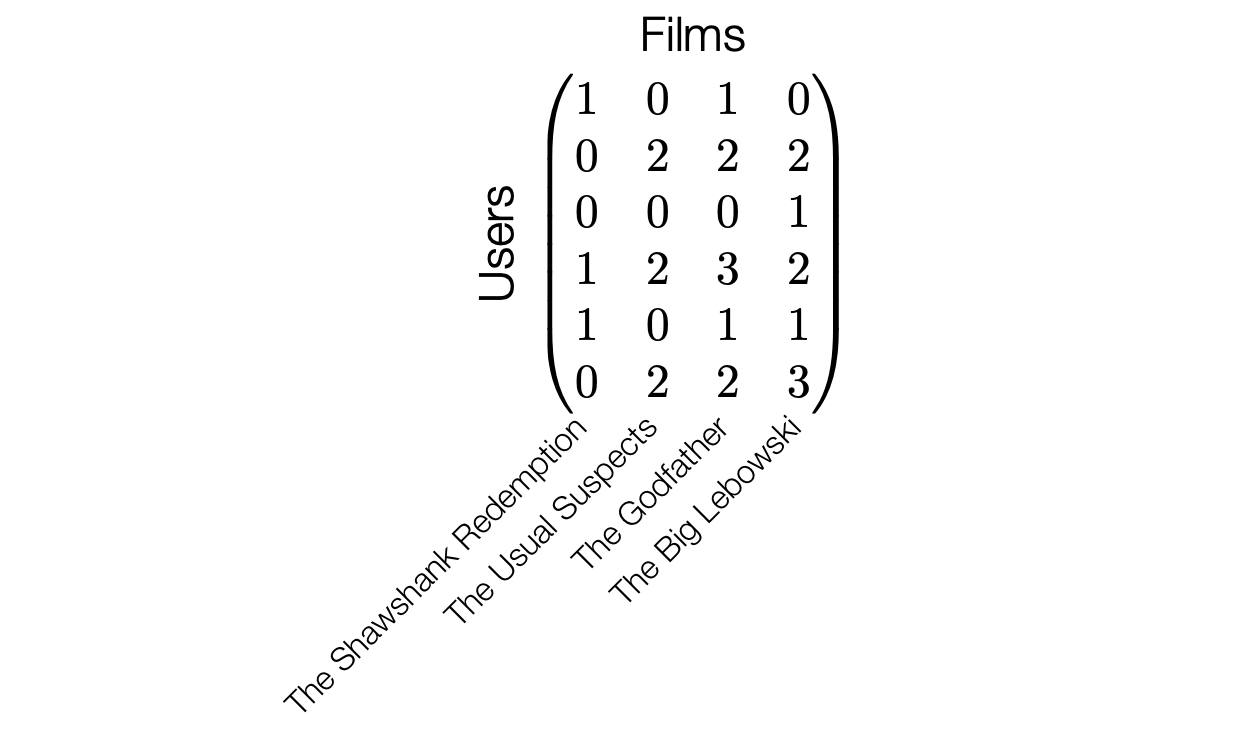
\includegraphics[scale=0.6]{images/predTask.png}
    \caption{esempio di task predittivo}
    \label{fig:enter-label}
\end{figure}

Le colonne rappresentano i film e le righe i giudizi delle persone ai quei film. Così è difficile tirare fuori qualche informazione utile, dobbiamo provare a generalizzare.

\begin{figure}[!h]
    \centering
    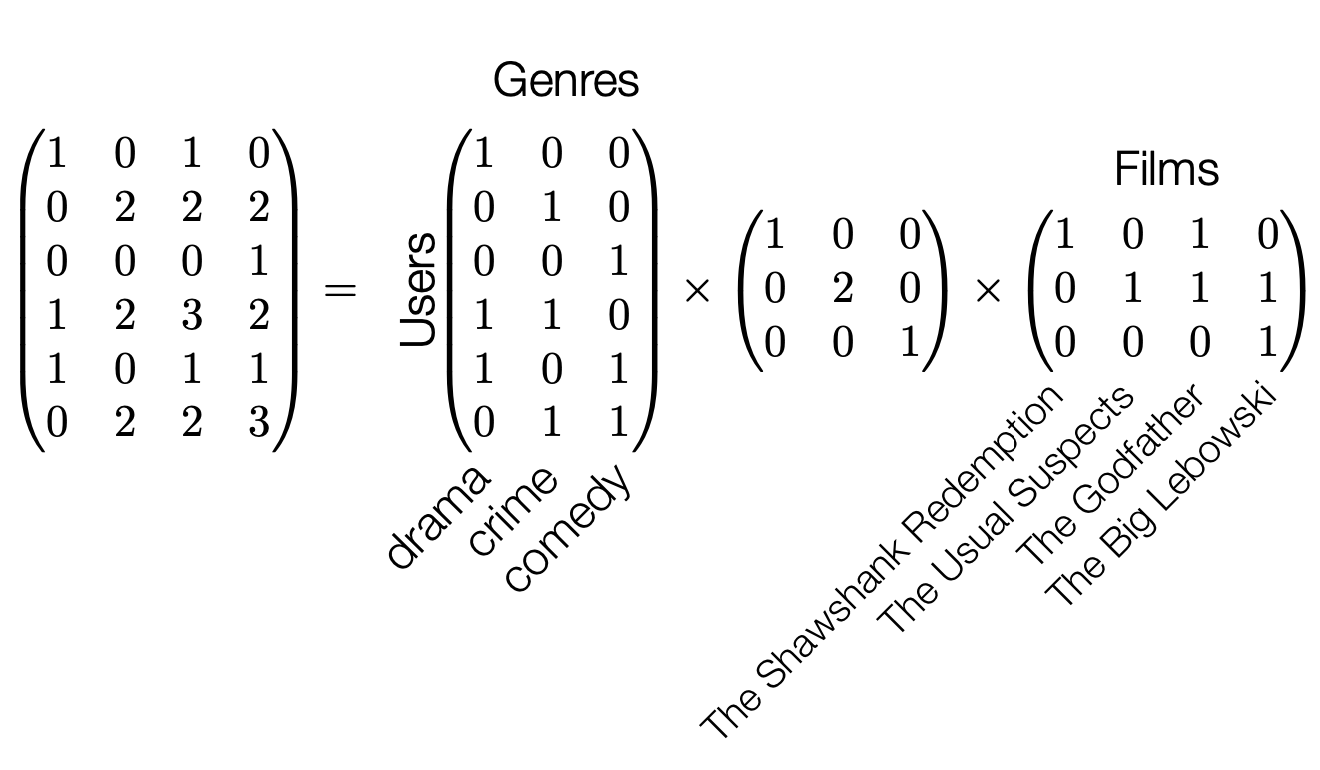
\includegraphics[scale=0.6]{images/predTask1.png}
    \caption{}
    \label{fig:enter-label}
\end{figure}

In questo modo è molto più semplice capire se ci sono relazioni tra gli utenti e i film.

\newpage

\section{Modelli} Vedremo 3 tipi di modelli:
\begin{itemize}
    \item \textbf{geometrici}, in cui si usano le intuizioni della geometria per risolvere il problema;
    \item \textbf{probabilistici}, in cui il tool principale è il calcolo della probabilità e la statistica;
    \item \textbf{logici}, in cui il tool principale sono le espressioni logiche.
\end{itemize}

In \textbf{ambito geometrico} un algoritmo di apprendimento deve \textbf{trovare l'insieme dei pesi} che permetta alla funzione di discriminare gli esempi.
\begin{equation}
    f_w(x)=w_1x_1+w_2x_2+w_3
\end{equation}
In questo esempio i pesi sono $w_1, w_2, w_3$ e gli algoritmi saranno algoritmi di ottimizzazione di qualche tipo.

\paragraph{Modelli probabilistici} Un classificatore di questo tipo, usa al posto della geometria, il calcolo della probabilità di un'etichetta avendo dei dati. Sia $X$ la descrizione del nostro esempio e $Y$ l'etichetta che vogliamo predire, quello che vorremmo fare è trovare $Y_{MAP}$ (cioè il massimo a posteriori), cioè la probabilità massima una volta che ho visto i dati.
\begin{equation}
\begin{split}
    Y_{MAP} = arg\; max_Y P(Y|X) \\
            = arg\; max_Y \frac{P(X|Y)P(Y)}{P(X)} \\
            = arg\; max_Y P(X|Y)P(Y)
\end{split}
\end{equation}
\textbf{Nota:} $P(Y|X)$ è la probabilità di avere $Y$ dato $X$.

Il denominatore non è importante perchè siamo interessati alla $Y$ che massimizza la probabilità.

Spesso $P(Y)$ non è nota quindi si usa la formula
\begin{equation}
    Y_{ML} = arg\; max_Y P(X|Y).
\end{equation}

Man mano che cresce il numero di valori da considerare, la tabella che viene fuori da questa formula è enorme (per $20$ valori sarebbero $2^{20}$ righe). In questo caso si usa uno degli algoritmi più semplici che si utilizzano con i metodi probabilistici è l'algoritmo di \textbf{Naive Bayes} che consiste nel fare un'assunzione forte su come sono fatte le probabilità (esempio assumere che $x_1$ e $x_2$ siano indipendenti tra di loro, quindi non serve calcolare l'intera tabella ma solo una per $x_1$ e una per $x_2$). 

\paragraph{Modelli logici.} Sono quei modelli in cui lo strumento che si utilizza per modellare i dati e i risultati è la \textbf{logica}. Ce ne sono molti tipi, un esempio è un classificatore logico che ha una serie di regole della forma se x allora y.
\begin{itemize}
    \item se l'email contiene la parola "viagra" stima gli odd di spam come 4:1 (spam e 4 volte più probabile rispetto ad ham);
    \item se l'email contiene la parola "blue pill" stima gli odd di spam come 3:1;
    \item altrimenti stima gli odd come 1:6.
\end{itemize}
Quindi quando si riceve un'email si applicano una dopo l'altra queste regole e la prima che matcha da la stima degli odd da cui poi si decide se dare spam o ham come etichetta corretta.

\section{Features}
Rappresentano come descriviamo i dati e hanno importanza fondamentale per arrivare ad un buon risultato. Facciamo un esempio

Supponiamo di voler approssimare $y = \cos{\pi x} $ nell'intervallo $-1 \le x \le 1$. Un'approssimazione lineare non sarebbe molto utile in questo caso, poiché il miglior adattamento sarebbe $y = 0$. Tuttavia, se suddividiamo l'asse $x$ in due intervalli, $-1 \le x < 0$ e $0 \le x \le 1$, possiamo trovare approssimazioni lineari ragionevoli in ciascun intervallo. Possiamo ottenere ciò utilizzando x sia come caratteristica di divisione che come variabile di regressione.

Un altro esempio: si vede che l'andamento è molto frastagliato.
\begin{figure}[!h]
    \centering
    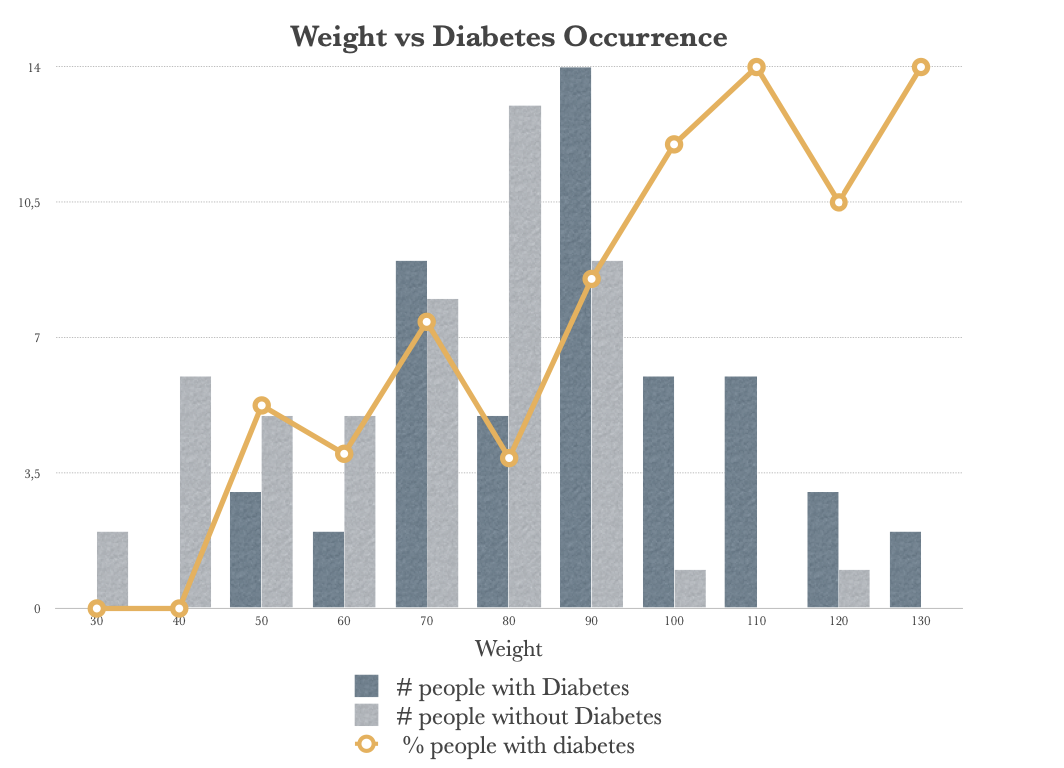
\includegraphics[scale=0.5]{images/diabetes0.png}
    \caption{Caption}
    \label{fig:enter-label}
\end{figure}

Se al posto di aggregare per 10 chili lo facciamo per 20 chili, si riesce a trattare molto meglio.
\begin{figure}[!h]
    \centering
    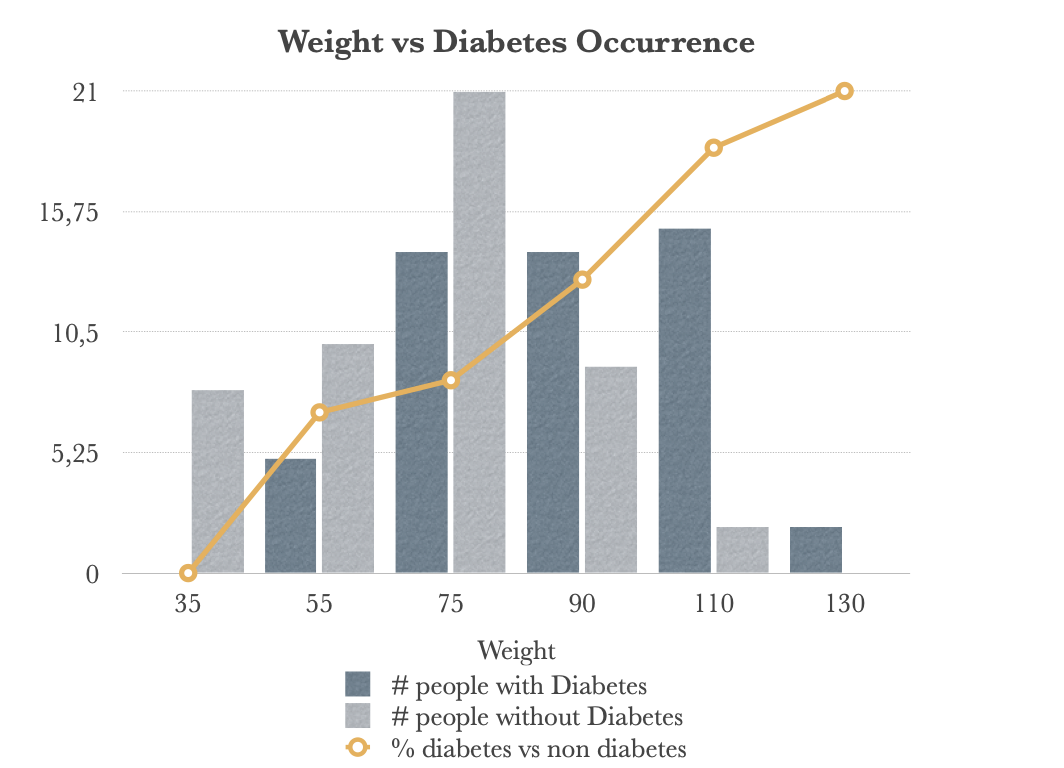
\includegraphics[scale=0.5]{images/diabetes1.png}
    \caption{Caption}
    \label{fig:enter-label}
\end{figure}

\textbf{Quindi anche solo lavorando sulle features, si riesce a semplificare di molto il problema.}